\section{Detection NA and detector sampling}

The next question was whether more information could be captured per illumination image. The detector study varied detection NA over 0.1, 0.2 and 0.3 and detector size over 12\ensuremath{\times}12, 24\ensuremath{\times}24 and 48\ensuremath{\times}48. It kept the random phase plate and learned solver, tuned each configuration separately, and tested two fixed scalar-measurement counts: M=36,864 and M=4,608. Increased light collection from higher NA was not credited through a separate throughput advantage in the noise convention.

\par\medskip\noindent\begin{minipage}{\linewidth}
\captionof{table}{Detection NA and spatial sampling at fixed scalar-measurement counts; random plate and learned prior.}
\centering
\begin{tabular}{@{}>{\raggedright\arraybackslash}p{0.176000\linewidth}@{\hspace{0.03\linewidth}}>{\raggedright\arraybackslash}p{0.176000\linewidth}@{\hspace{0.03\linewidth}}>{\raggedright\arraybackslash}p{0.176000\linewidth}@{\hspace{0.03\linewidth}}>{\raggedright\arraybackslash}p{0.176000\linewidth}@{\hspace{0.03\linewidth}}>{\raggedright\arraybackslash}p{0.176000\linewidth}@{}}\toprule
Detection NA & Detector & Images at C=1 / C=8 & Depth at C=1 / C=8 (\ensuremath{\mu}m) & PSNR at C=1 / C=8 (dB) \\
\midrule
0.1 & 12\ensuremath{\times}12 & 256 / 32 & 0.346 / 0.475 & 33.19 / 32.09 \\
0.1 & 24\ensuremath{\times}24 & 64 / 8 & 0.368 / 0.613 & 33.13 / 31.36 \\
0.1 & 48\ensuremath{\times}48 & 16 / 2 & 0.437 / 1.261 & 32.48 / 28.82 \\
0.2 & 12\ensuremath{\times}12 & 256 / 32 & 0.302 / 0.425 & 33.88 / 32.60 \\
0.2 & 24\ensuremath{\times}24 & 64 / 8 & 0.281 / 0.439 & 34.37 / 32.85 \\
0.2 & 48\ensuremath{\times}48 & 16 / 2 & 0.312 / 0.969 & 34.36 / 30.22 \\
0.3 & 12\ensuremath{\times}12 & 256 / 32 & 0.297 / 0.419 & 34.05 / 32.61 \\
0.3 & 24\ensuremath{\times}24 & 64 / 8 & 0.281 / 0.428 & 34.49 / 32.94 \\
0.3 & 48\ensuremath{\times}48 & 16 / 2 & 0.314 / 0.834 & 34.73 / 31.32 \\
\bottomrule\end{tabular}
\end{minipage}\par\medskip


At C=1, NA 0.3 with a 48\ensuremath{\times}48 detector used 16 images and improved both mean PSNR and depth error relative to the original detector's 256-image result. At C=8, the 24\ensuremath{\times}24 high-NA configurations used eight images with mean depth error below the generic-prior baseline's full-measurement value. However, reducing to two images with a 48\ensuremath{\times}48 detector degraded depth substantially.

The key is the combination of optics and sampling. At NA 0.1, substituting more detector pixels for illumination directions made recovery worse. Higher NA passes more lateral detail and changes defocus-dependent detector responses; a finer detector can retain this information. This explains the observed spatial--temporal trade-off without treating extra pixels as free measurement compression.

The first NA-0.3 full-measurement tuning ended on a penalty-grid boundary. A wider search replaced those rows; the final changes were at most about 0.1 dB. The consolidated table uses the corrected selections. A 96\ensuremath{\times}96 option was not pursued because of footprint cost and limited expected benefit at the tested optical bandwidth.

\textbf{Conclusion:} more informative detection can replace many sequential images at fixed scalar-measurement count. The 16-image high-NA result is image-count reduction, not C=16 measurement compression.

Evidence: D24; final detector block, {\small\texttt{detector\_\allowbreak{}study/\allowbreak{}}} rows, including the edge-corrected selections.


\begin{figure}[htbp]
\centering
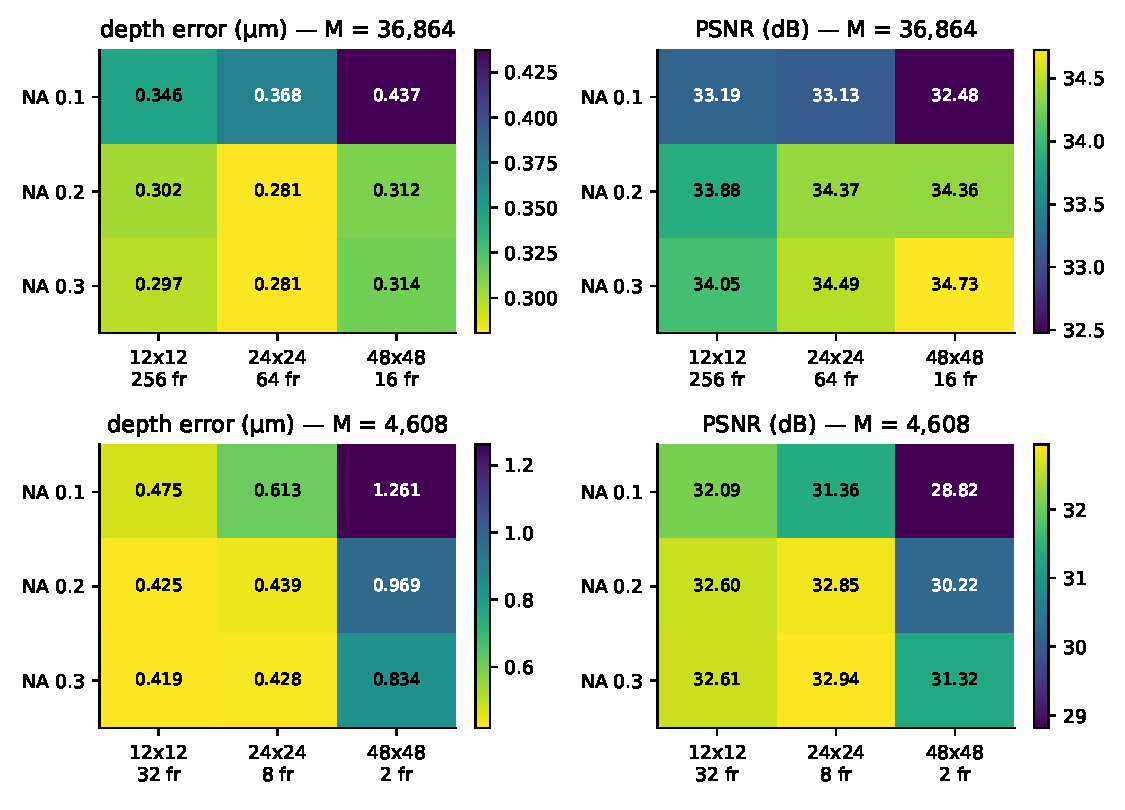
\includegraphics[width=\linewidth,height=0.57\textheight,keepaspectratio]{figures/detector_sampling.pdf}
\caption{Joint detection-NA and sampling study with the random plate and learned prior. Within each row of panels the scalar measurement count is fixed, while camera-image count changes with detector size. Values are means over eight test subvolumes. Panels have separate colour scales; compare their printed values.}
\label{exp:fig_detector_grid}
\end{figure}
\FloatBarrier
